%%
%% This is file `sample-manuscript.tex',
%% generated with the docstrip utility.
%%
%% The original source files were:
%%
%% samples.dtx  (with options: `manuscript')
%% 
%% IMPORTANT NOTICE:
%% 
%% For the copyright see the source file.
%% 
%% Any modified versions of this file must be renamed
%% with new filenames distinct from sample-manuscript.tex.
%% 
%% For distribution of the original source see the terms
%% for copying and modification in the file samples.dtx.
%% 
%% This generated file may be distributed as long as the
%% original source files, as listed above, are part of the
%% same distribution. (The sources need not necessarily be
%% in the same archive or directory.)
%%
%% The first command in your LaTeX source must be the \documentclass command.
%%%% Small single column format, used for CIE, CSUR, DTRAP, JACM, JDIQ, JEA, JERIC, JETC, PACMCGIT, TAAS, TACCESS, TACO, TALG, TALLIP (formerly TALIP), TCPS, TDSCI, TEAC, TECS, TELO, THRI, TIIS, TIOT, TISSEC, TIST, TKDD, TMIS, TOCE, TOCHI, TOCL, TOCS, TOCT, TODAES, TODS, TOIS, TOIT, TOMACS, TOMM (formerly TOMCCAP), TOMPECS, TOMS, TOPC, TOPLAS, TOPS, TOS, TOSEM, TOSN, TQC, TRETS, TSAS, TSC, TSLP, TWEB.
% \documentclass[acmsmall]{acmart}
\documentclass[sigchi,authordraft]{acmart}

%% 追加
\usepackage{bm}
\newcommand\figref[1]{\textbf{Figure~\ref{fig:#1}}}
\newcommand\tabref[1]{\textbf{Table~\ref{tab:#1}}}
\usepackage{url}
\usepackage{color}
\usepackage{multirow}
%% ここまで

%%%% Large single column format, used for IMWUT, JOCCH, PACMPL, POMACS, TAP, PACMHCI
% \documentclass[acmlarge,screen]{acmart}

%%%% Large double column format, used for TOG
% \documentclass[acmtog, authorversion]{acmart}

%%%% Generic manuscript mode, required for submission
%%%% and peer review
% \documentclass[manuscript,screen,review]{acmart}
%% Fonts used in the template cannot be substituted; margin 
%% adjustments are not allowed.
%%
%% \BibTeX command to typeset BibTeX logo in the docs
\AtBeginDocument{%
  \providecommand\BibTeX{{%
    \normalfont B\kern-0.5em{\scshape i\kern-0.25em b}\kern-0.8em\TeX}}}

%% Rights management information.  This information is sent to you
%% when you complete the rights form.  These commands have SAMPLE
%% values in them; it is your responsibility as an author to replace
%% the commands and values with those provided to you when you
%% complete the rights form.
\setcopyright{acmcopyright}
\copyrightyear{2018}
\acmYear{2018}
\acmDOI{10.1145/1122445.1122456}

%% These commands are for a PROCEEDINGS abstract or paper.
\acmConference[Woodstock '18]{Woodstock '18: ACM Symposium on Neural
  Gaze Detection}{June 03--05, 2018}{Woodstock, NY}
\acmBooktitle{Woodstock '18: ACM Symposium on Neural Gaze Detection,
  June 03--05, 2018, Woodstock, NY}
\acmPrice{15.00}
\acmISBN{978-1-4503-XXXX-X/18/06}


%%
%% Submission ID.
%% Use this when submitting an article to a sponsored event. You'll
%% receive a unique submission ID from the organizers
%% of the event, and this ID should be used as the parameter to this command.
%%\acmSubmissionID{123-A56-BU3}

%%
%% The majority of ACM publications use numbered citations and
%% references.  The command \citestyle{authoryear} switches to the
%% "author year" style.
%%
%% If you are preparing content for an event
%% sponsored by ACM SIGGRAPH, you must use the "author year" style of
%% citations and references.
%% Uncommenting
%% the next command will enable that style.
%%\citestyle{acmauthoryear}

%%
%% end of the preamble, start of the body of the document source.
\begin{document}

%%
%% The "title" command has an optional parameter,
%% allowing the author to define a "short title" to be used in page headers.
\title{disp2ppg: Pulse Wave Generation to PPG Sensor using Display}

%%
%% The "author" command and its associated commands are used to define
%% the authors and their affiliations.
%% Of note is the shared affiliation of the first two authors, and the
%% "authornote" and "authornotemark" commands
%% used to denote shared contribution to the research.

% \author{Atsuhiro Fujii}
% \affiliation{%
%   \institution{Ritsumeikan University}
%   \city{Shiga}
%   \country{Japan}}
% \email{atsuhiro.fujii@iis.ise.ritsumei.ac.jp}

% \author{Kazuya Murao}
% \affiliation{%
%   \institution{Ritsumeikan University}
%   \city{Shiga}
%   \country{Japan}}
% \email{murao@cs.ritsumei.ac.jp}

%%
%% By default, the full list of authors will be used in the page
%% headers. Often, this list is too long, and will overlap
%% other information printed in the page headers. This command allows
%% the author to define a more concise list
%% of authors' names for this purpose.
% \renewcommand{\shortauthors}{Fujii and Murao}

%%
%% The abstract is a short summary of the work to be presented in the
%% article.
\begin{abstract}
  Research on wearable devices has been actively conducted, and devices of various shapes and wearing areas have been proposed. 
  Wearable devices are often used to record the user's biometric information, and methods to detect physical abnormalities from the acquired data have been proposed. Among biometric data, pulse data has been used in methods such as emotion estimation. The most common type of pulse sensor is the PPG (Photoplethysmogram), which irradiates a green LED on the skin and measures pulse data from the changes in the light reflected through the blood vessels. PPG sensors have been introduced into commercially available wearable devices such as smartwatches. The PPG sensor requires blood flow for data acquisition due to the characteristics of the mechanism. When a smartwatch is worn on an artificial body such as a prosthetic hand or a wearable robot arm, correct data cannot be acquired because there is no blood flow. In this study, we propose a method to make the PPG sensor measure arbitrary pulse data using a display. If this method is realized, it will be possible to input pulse data measured at the junction of the live body and the prosthetic hand to the display, and have the smartwatch attached to the prosthetic hand read same pulse data. In this paper, we focus on the heart rate, and describe the results of an experiment in which the target heart rate was input and the display was controlled, and whether the target heart rate could be obtained by a smartwatch worn on the display. We implemented a display drawing program and conducted an evaluation experiment using five kinds of smartwatches and four kinds of displays to confirm the effectiveness of the proposed method. As a result, the overall error between the target heart rate entered and the heart rate acquired by the smartwatch was within -3 beats per minute in most cases.
\end{abstract}

%%
%% The code below is generated by the tool at http://dl.acm.org/ccs.cfm.
%% Please copy and paste the code instead of the example below.
%%
% \begin{CCSXML}
% <ccs2012>
%  <concept>
%   <concept_id>10010520.10010553.10010562</concept_id>
%   <concept_desc>Computer systems organization~Embedded systems</concept_desc>
%   <concept_significance>500</concept_significance>
%  </concept>
%  <concept>
%   <concept_id>10010520.10010575.10010755</concept_id>
%   <concept_desc>Computer systems organization~Redundancy</concept_desc>
%   <concept_significance>300</concept_significance>
%  </concept>
%  <concept>
%   <concept_id>10010520.10010553.10010554</concept_id>
%   <concept_desc>Computer systems organization~Robotics</concept_desc>
%   <concept_significance>100</concept_significance>
%  </concept>
%  <concept>
%   <concept_id>10003033.10003083.10003095</concept_id>
%   <concept_desc>Networks~Network reliability</concept_desc>
%   <concept_significance>100</concept_significance>
%  </concept>
% </ccs2012>
% \end{CCSXML}

% \ccsdesc[500]{Computer systems organization~Embedded systems}
% \ccsdesc[300]{Computer systems organization~Redundancy}
% \ccsdesc{Computer systems organization~Robotics}
% \ccsdesc[100]{Networks~Network reliability}

%%
%% Keywords. The author(s) should pick words that accurately describe
%% the work being presented. Separate the keywords with commas.
\keywords{ppg sensor, display, pulse wave, heart rate, smartwatch}

%% A "teaser" image appears between the author and affiliation
%% information and the body of the document, and typically spans the
%% page.
% \begin{teaserfigure}
%   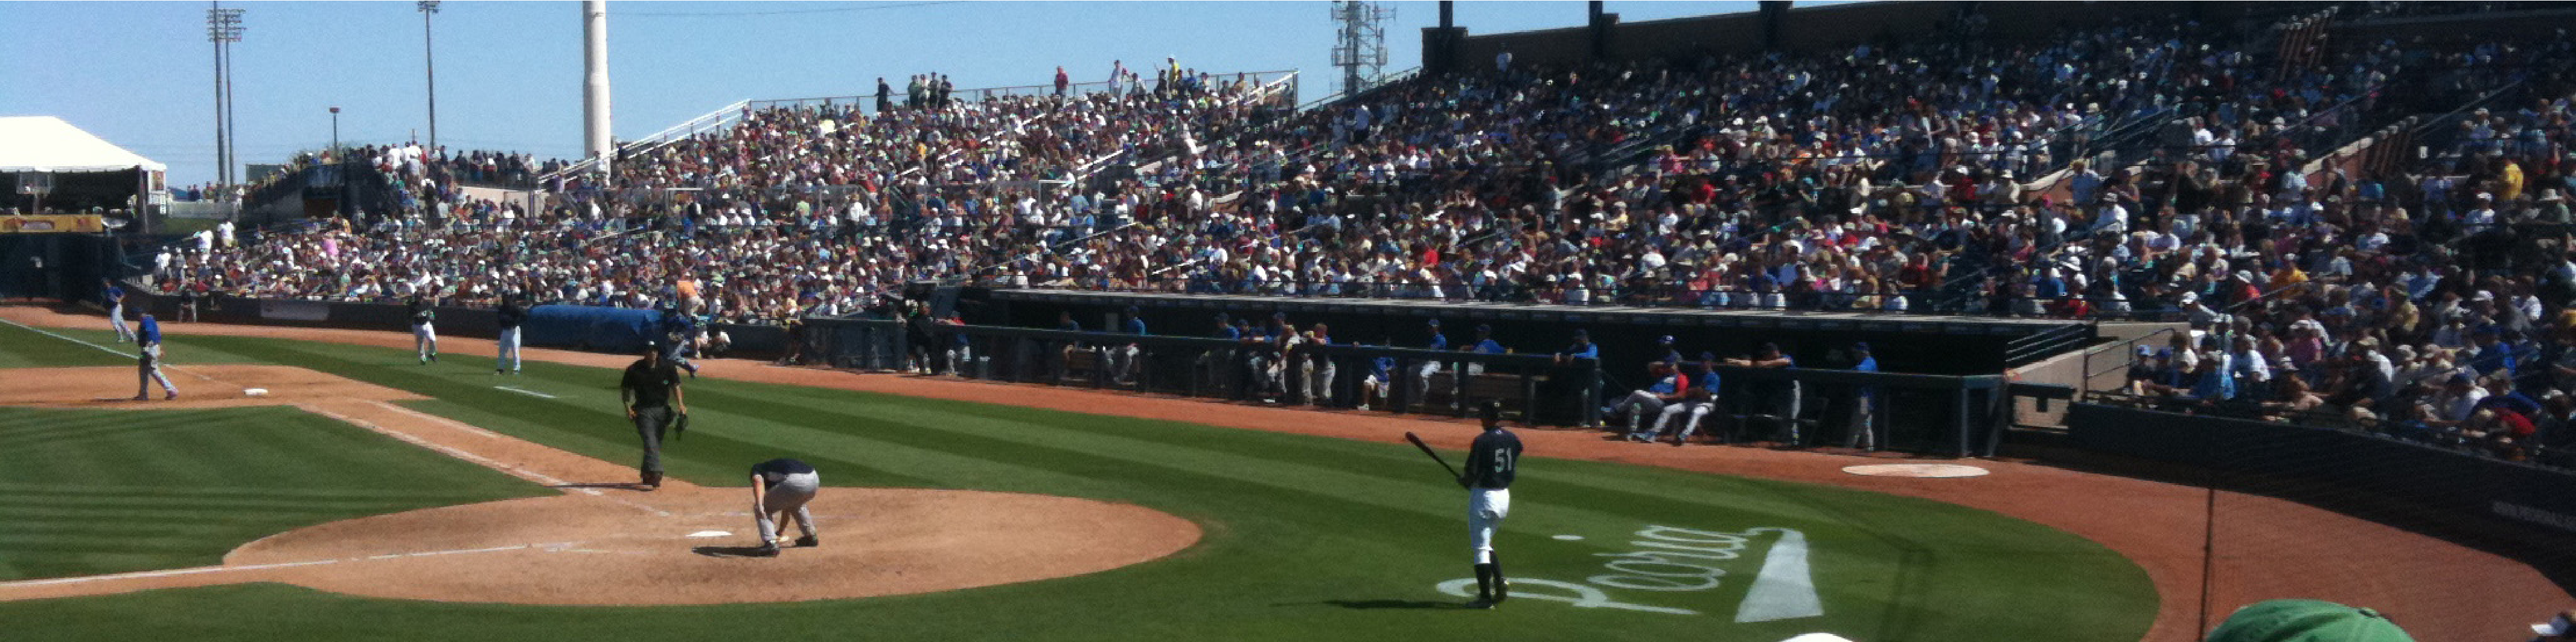
\includegraphics[width=\textwidth]{sampleteaser}
%   \caption{Seattle Mariners at Spring Training, 2010.}
%   \Description{Enjoying the baseball game from the third-base
%   seats. Ichiro Suzuki preparing to bat.}
%   \label{fig:teaser}
% \end{teaserfigure}

%%
%% This command processes the author and affiliation and title
%% information and builds the first part of the formatted document.
\maketitle

% 1
\section{Introduction}
\label{sec:introduction}
With the growing awareness of health management, wearable devices that record biometric information have become widely used. The biometric information to be recorded includes a variety of information such as activity, respiratory rate, body temperature, cardiac potential, blood pressure, gaze, etc. The pulse wave and the heart rate are among them. The pulse sensor used to acquire the pulse waves and the heart rate irradiates the skin with LEDs that emit infrared, red light, or light with a green wavelength around 550 nm. The oxidized hemoglobin in the blood of arteries has the property of absorbing these lights. The pulse sensor utilizes the fact that the amount of reflected light decreases as the arterial blood flow increases with the timing of the heartbeat, and uses a phototransistor to acquire changes in the amount of reflected light and measure the pulse wave. The pulse wave data is numerical data of the change of the reflected light, and the heart rate is measured by detecting the peak appearing in the pulse wave data. This types of pulse wave measurement method is called PPG (Photoplethysmogram). Many commercially available wearable devices, such as smartwatches, are equipped with PPG sensor as a pulse sensor. 

% Havriushenko et al.\cite{respiratory_rate_estimation} proposed a method for estimating respiratory rate using pulse wave data. The pulse wave is one of the most important pieces of biometric data, and research using pulse wave data is flourishing.\par

We consider the possibility of measuring an arbitrary pulse wave by giving a change of light to the PPG sensor and in this paper we propose disp2ppg, a method to let the PPG sensor to acquire pulse data using a display. The proposed method makes a smartwatch to measure an arbitrary heart rate. We assume two objectives for disp2ppg: PPG transfer and fake PPG.

As an application of PPG transfer, artificial bodies, such as prosthetic hands, wearable robot arms, and telepresence robot do not have blood flow. Therefore, it is not possible to measure the biometric data even if a smartwatch is worn on the wrist. Smartwatch functions such as calling, messaging, clocking, and payment, as well as sensors such as accelerometers and GPS, can be used in artificial bodies as in the living body, but pulse data cannot be measured. When a smartwatch is forcibly attached to other body parts where blood flow exists, such as the ankle, in order to measure pulse data, the usability of other functions, such as the messaging, is reduced.
%Currently, if one wishes to measure pulse waves in an artificial body, it is necessary to attach an additional pulse wave sensor to a body part where pulse wave data can be measured, and to collect data by communicating with a smartphone or similar device. In a situation where a shopkeeper and a customer are separated by an acrylic panel and communicate through a hole in the acrylic panel, it is not possible to have the shopkeeper measure the body temperature with an artificial body through the hole. 
With the proposed method, even when a smartwatch is attached to an artificial body, the smartwatch can read the person's pulse data by changing the light of the display under the PPG sensor of the smartwatch according to the pulse data measured at the junction of the living body and the prosthetic hand. It is possible to use the functions provided by a smartwatch since the smartwatch is not modified and only the display is mounted on the artificial body. Users can compare various items such as design, function, and weight of commercial smartwatches and use the model of his/her choice. When applied to a remote robot avatar, the operator's biometric data can be measured on the avatar's body.\par

As an application of fake PPG, it is possible to let the PPG sensor to measure an arbitrary heart rate by the proposed method and a malicious user could falsify the heart rate and pretend to exercise or continue resting. If a device that realizes the proposed method becomes widely feasible and has a significant social impact, it will be necessary to discuss the use of the current PPG sensor from the viewpoint of the vulnerability of the PPG sensor.\par

% In the following sections, we introduce related works in Section \ref{sec:related} and explain the details of the proposed method in Section \ref{sec:method}. Section \ref{sec:evaluation} discusses the evaluation of the proposed method, Section \ref{sec:future_work} describes our future plans, and finally Section \ref{sec:conclusion} concludes the paper.



% 2
\section{Related Work}
\label{sec:related}
%This section introduces research on sensing with wearable devices, the use of smart watches, and the use of pulse data.

% 2.1
%\subsection{Sensing with wearable devices}
%Ham et al.\cite{smart_wristband} have proposed a wristband-type device as an input device for smart glasses. This device is equipped with a touch panel and an inertial measurement unit, and can be operated by touch or a motion such as a twist of the wrist. Since the device can be used by wearing it on the wrist, the user's movement is not restricted and has a high degree of freedom. A touch panel was used for pointing to improve the stability of the input.
%Hernandez et al.\cite{bioglass} propose a method for recognizing pulse rate and respiration rate from data obtained from the accelerometer, gyroscope, and camera built into Google Glass, a head-worn wearable device.
%Nishajith et al.\cite{smart_cap} designed and implemented Smart Cap as a wearable device to assist the visually impaired with situational awareness. The device consists of a Raspberry Pi 3, a Raspberry Pi NoIR Camera V2, an earphone, and a power supply. The Raspberry Pi NoIR (No Infrared) Camera V2 is an infrared camera module for the Raspberry Pi. The object detected in the image obtained by this infrared camera is described by voice through an earphone.
%These are all researches on wearable devices that are worn on body parts, and researches using devices of various shapes have been conducted.\par

% There are various body parts where wearable devices are worn.
% Vahdatpour et al.\cite{localization_vahdatpour} had 25 subjects wear accelerometers at 10 locations on the forearm, upper arm, head, thigh, shin, and waist, and collected acceleration data during daily activities. From the collected data, the SVM (Support Vector Machine) was used to estimate the attachment site with an average accuracy of 89\%.
% Sztyler et al.\cite{localization_sztyler} attached accelerometers to seven locations on the head, chest, left upper arm, left wrist, waist, left pocket of pants, and left ankle of 15 subjects and collected acceleration data during various physical activities. From the collected data, the wearing site was estimated using Random Forest, and an average accuracy of 89\% was achieved.
% Kunze et al.\cite{localization_kunze} attached accelerometers to four locations on the wrist, the right side of the head above the eyes, the left trouser’s pocket, and the left breast pocket of six subjects and collected data during walking movements. From the collected data, the attachment site was estimated using the C4.5 classifier.
% We have proposed a method to estimate the body part where the wearer is wearing a wearable device without having the wearer perform a specific action, using ECG and pulse data, which are biometric information that can be acquired by the wearable device.\cite{localization_yoshida}\par

% As described above, wearable devices have been proposed in various shapes. Because of the wide range of wearing sites, research using wearable devices has been actively conducted.


% 2.2
\subsection{Studies using Smartwatch}
Smartwatches have been commercially available for a long time and many researches using a smartwatch have been conducted.
%Spinsante et al.\cite{accuracy_in_low_intensity} focused on the heart rate obtained from a smartwatch during low-intensity physical activity and measured its accuracy.
Sen et al.\cite{eating_recognition} proposed a method to record eating behavior, such as whether the user ate with hands, chopsticks, or a spoon, using data obtained from the accelerometer and gyroscope of a smartwatch. 
Johnston et al.\cite{smartwatch_walk_authentication} proposed a method for biometric authentication based on gait using data obtained from the accelerometer and gyroscope of the smartwatch.
%Weiss et al.\cite{smartwatch_activity_recognition} showed that a smartwatch can identify actions more effectively than a smartphone in hand-based physical behaviors such as eating. For the behavior ``drinking'', the smartwatch was able to identify the behavior with 93.3\% accuracy, while the smartphone could only achieve 77.3\% accuracy.
Iakovakis et al.\cite{oh_detection} conducted a study that predicts the blood pressure drop caused by postural changes using a smart watch. 
Mauldin et al.\cite{smartfall} proposed an Android application ``SmartFall'' that detects falls using acceleration data obtained from a commercially available smartwatch. 
%Ciabattoni et al.\cite{smartwatch_stress_detection} have proposed a method for detecting mental stress during various cognitive tasks in real time. Galvanic Skin Response (GSR), RR Interval and Body Temperature (BT) acquired by a commercial smartwatch are used to classify stress.\par
These methods using inertia sensors such as accelerometers are applicable even with artificial body, however, methods using pulse data are unavailable.
%We try to make these applications available to artificial bodies as well as to living bodies by inputting data to biometric sensors of wearable devices.

% 2.3
\subsection{Studies using Pulse Data}
There have been proposed several methods and applications using pulse data.
Havriushenko et al.\cite{respiratory_rate_estimation} proposed a method for estimating respiratory rate from pulse wave data using neural networks. %To measure respiratory rate, thermal sensor placed in nasal channels or elastic chest belt are often used. However, these devices may interfere with sleep. A method of measuring respiratory rate using pulse wave data can be implemented in a wearable device. As a result of the evaluation, the proposed model provides an average respiratory rate estimation error lower than 2.2 breaths per minute.
Han et al.\cite{arrhythmia_detection} proposed a method for detecting premature atrial contraction (PAC) and premature ventricular contraction (PVC) using PPG data acquired from a smartwatch.
Goshvarpour et al.\cite{emotion_recognition_poincare} proposed a method for classifying emotional responses with the electrocardiogram and finger pulse activity. % of 35 participants during rest condition and when subjects were listening to music intended to stimulate certain emotions. After using poincare plots, the SVM was used to classify them into four emotions: happiness, sadness, peacefulness, and fear.
Kajiwara et al.\cite{pulse_order_picking} focused on the fact that many logistics companies adopt a manual order picking system, and that emotions and engagement affect work efficiency and human errors, and proposed a method for predicting emotions and engagement during work with high exercise intensity based on behavior and pulse waves acquired by wearable devices. %Pulse wave, eye movements, and movements are input to deep neural networks to estimate emotion and engagement. The results of verification experiments showed that emotion and engagement during order picking can be predicted from the behavior of the worker with an accuracy of error rate of 0.12 or less.
Lee et al.\cite{fast_emotion_recognition} conducted research on improving the speed of emotion recognition using PPG signal. %A two-dimensional emotion model based on valence and arousal is adopted, and one-dimensional convolutional neural network (1D CNN) is used to recognize emotion from 1.1 second PPG signal. They tested the 1D CNN as a binary classification (high or low valence and arousal) using the dataset for emotion analysis using physiological (DEAP) signals, and achieved recognition accuracy of 75.3\% for valence and 76.2\% for arousal.\par
Pulse data is one of the most important biological information, as it can detect abnormalities in the body and estimate emotions. Most of the pulse sensors in commercially available wearable devices use photoplethysmogram. Therefore, when a wearable device is worn on an artificial body where blood flow does not exist, pulse data cannot be acquired. We propose a method to let a wearable device to measure pulse data similar to that of a living body even on an artificial body.

% 3
\section{Proposed Method}
\label{sec:method}
This section explains the details of the proposed method.

% 3.1
\subsection{Overview}
\label{subsec:overview}
%When a user sets an arbitrary heart rate, the proposed method changes the color of the display and a smartwatch worn on the display measures the specified heart rate. 
The flow of the proposed method is shown in \figref{method}. First, the real and target heart rate of the user is obtained with PPG sensor which is different to the smartwatch. The proposed method changes the brightness of the display connected to a microcomputer according to the target heart rate. Then, the smartwatch worn over the display measures the heart rate which is the same as the target heart rate.\par

\begin{figure}[!t]
  \centering
  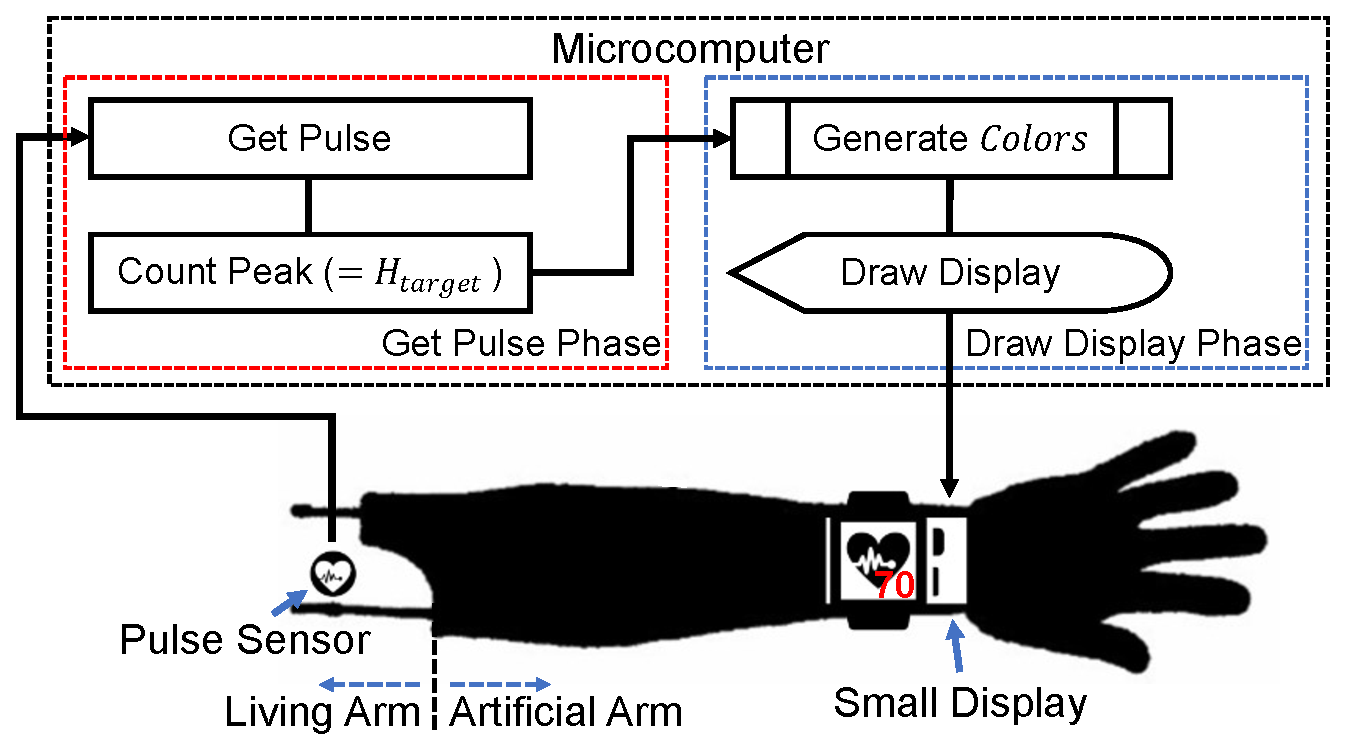
\includegraphics[width=1\linewidth]{figures/method.eps}
  \caption{Process flow of the proposed method.}
  \label{fig:method}
\end{figure}

% 3.2
\subsection{Target Heart Rate Calculation}
The target heart rate that the proposed method lets the smartwatch to measure is the wearer's heart rate obtained using another PPG sensor, and that value can be specified in real time. Let $H_{target}$ be the target heart rate. $H_{target}$ can also be given manually if the user want the smartwatch to measure specific heart rate.

% 3.3
\subsection{Display Control}
\label{subsec:display_control}
The brightness of the display is controlled so that the heart rate measured by the smartwatch becomes $H_{target}$. An array $Colors$ that holds the brightness of the display to let the smartwatch to detect a single pulse is prepared in advance.
% Through the preliminary investigation, $Colors$ was determined to the following sequence of numbers. 
% \begin{equation*}
%   \begin{split}
%     Colors = [255, 255, 255, 255, 255, 255, 255, 255, 255, 255,\\250, 240, 232, 227, 225, 225, 229, 236, 245, 255]
%   \end{split}
% \end{equation*}
$Colors$ is grayscale data. Grayscale is a type of computer color representation that uses 256 levels (0-255) to represent shades of color from black to white. $Colors$ whose length is $L$ is generated in the following flow.
\begin{enumerate}
  \renewcommand{\labelenumi}{\arabic{enumi}.}
  \item $Colors[i]=\sin\left(\frac{2\pi i}{L}\right)~(i=0,\dots,L)$
  \item $Colors[i]=Colors[i]+1$
  \item $Colors[i]=1$ (if $Colors[i]>1$)
  \item $Colors[i]=Colors[i]*SCALE+BASE$
\end{enumerate}
\figref{colors_wave} shows the plot of $Colors$ when $L$, $SCALE$, and $BASE$ are set to 30, 19, 225. PPG sensors irradiates infrared, red or green LEDs onto the skin and measures pulse data from the changes in light reflected through the blood vessels. Because blood flow increases with the timing of the pulse, more light is absorbed by the blood vessels, and the reflected light is dimmer. The decreasing values in  \figref{colors_wave} represent the timing when the reflected light becomes dark. The smaller the grayscale, the closer it is to black. Since black absorbs more light than white, the more the display is rendered black, the darker the light emitted from the smartwatch worn on the display and reflected through the display.\par

\begin{figure}[!t]
  \centering
  \includegraphics[width=1\linewidth]{figures/colors_wave.eps}
  \caption{Time-series brightness of the display that makes a smartwatch detect a single pulse.}
  \label{fig:colors_wave}
\end{figure}

The drawing interval $T$[s] for each value of $Colors$ is set as follows so that $Colors$ is played $H_{target}$ times in one minute.
\begin{equation}
  \label{eqn:wait}
  T = \frac{60}{L * H_{target}}
\end{equation}
The proposed method draws the values of $Colors$ on the display $T$[s] one by one for each.


% 3.4
\subsection{Pulse Data Measurement}
In the proposed method, a smartwatch is worn over a blinking display and pulse data is measured. Pulse data measured from a PPG sensor equipped on a smartwatch can be used in various applications. However, the performance of the PPG sensor and the algorithm for measuring the pulse data vary depending on the model of the smartwatch equipped with it, and are not disclosed to the public. Therefore, the target heart rate is set manually in the evaluation experiment. We observe the error between the target heart rate and the heart rate measured by the smartwatch, and discuss the effects of the smartwatch model and display.

% 4
\section{Evaluation}
\label{sec:evaluation}
This section describes the experiments conducted to evaluate the effectiveness of the proposed method. We measured the heart rate acquired by the smartwatch when an arbitrary target heart rate was given.

% 4.1
\subsection{Display Control Software}
\label{subsec:software}
A program to change the brightness of the display was implemented using Python and Processing\footnote{\url{https://processing.org}}. 
%Processing\footnote{\url{https://processing.org}} is a programming language based on Java that excels in visual expression, and is used to create electronic art and visual design. The process flow of the implemented program is shown below. 
First, Python receives the target heart rate $H_{target}$. 
%In the color data creation part, we use Numpy\footnote{\url{https://numpy.org}} to create $Colors$. 
Then, $T$[s] is calculated with Eqn. \ref{eqn:wait}. The Python sends $Colors[i]$ to Processing using Python's \texttt{socket} library and waits for the drawing to complete. When Processing receives the data, it uses \texttt{background} method to draw the grayscale as the background color of the window on the display. When drawing is completed, Python receives the notification from Processing. If $T$[s] has passed, Python sends $Colors[i+1]$ to Processing. When all the data in $Colors$ has been sent, $H_{target}$ is obtained and the system repeats this flow.

% 4.2
\subsection{Smartwatch Application}
\label{subsec:wearos}
A smartwatch is used to measure the heart rate. Smartwatches have different methods of acquiring heart rate depending on the operating system installed on them. In this section, we describe the methods of obtaining the heart rate for each OS.
% However, the application initially installed on the smartwatch stops sensing and turns off the screen after a certain period of time, and the heart rate cannot be saved as a numerical value, therefore we implemented a smartwatch application that logs the heart rate.\par


% 4.2.1
\subsubsection{Wear OS by Google}
TicWatch Pro WF12106 and PUMA Smartwatch were used in the evaluation experiment. These are a smartwatch with Wear OS by Google\footnote{\url{https://wearos.google.com}} which is an operating system designed for smartwatches based on Google's Android. We implemented the application using Android Studio\footnote{\url{https://developer.android.com/studio}}. The application stores heart rate in the smartwatch storage in csv format.
%The implemented application is shown in \figref{app}. When we start the application, the screen shown in (1) will be displayed. The acquisition of the sensor value starts automatically, and when there is a change in the value, the sensor value is displayed as shown in (2). ``Heart'' indicates the value of the heart rate sensor, and ``Pulse'' indicates the value of the PPG sensor. If we want to record the data, we press the ``RECORD'' button. Then, the 60-second calibration will start as shown in (3). This calibration waits for the value variation to stabilize. We will adjust the wearing position of the smartwatch during this time. When the 60-second calibration is completed, the sensor data is acquired for 60 seconds as shown in (4) and stored in a variable. At the end of the sensor data acquisition time, the data stored in the variable will be saved in the smartwatch storage in csv format, and a message indicating the completion of data acquisition will be displayed as shown in (5). 
%\tabref{sensor_param} shows the details of the sensors used in the implementation. 
The sensor number 21 is used to acquire the heart rate data. The rate of events ``SENSOR\_DELAY\_UI'' is used to set sampling rate suitable for the implementation of the user interface\footnote{\url{https://developer.android.com/reference/android/hardware/SensorManager}}.

% \begin{figure}[!t]
%   \centering
%   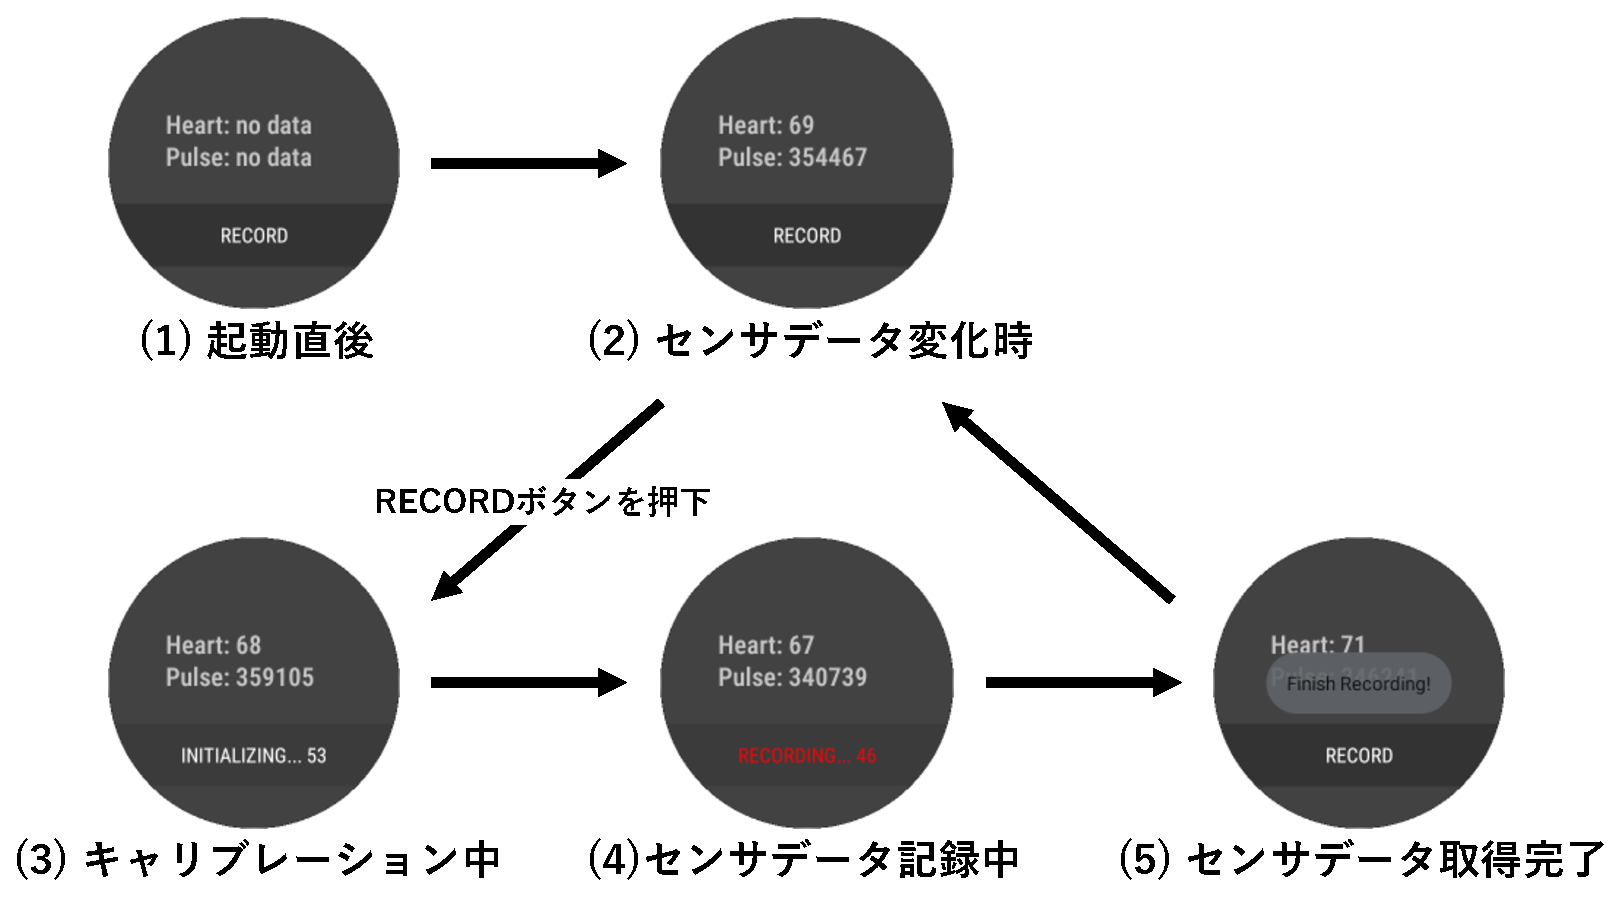
\includegraphics[width=1\linewidth]{figures/app.eps}
%   \caption{Details of the implemented application.}
%   \label{fig:app}
% \end{figure}

% \begin{table}[!t]
%   \centering
%   \caption{Details of the sensor used for wearOS implementation.}
%   \begin{tabular}{c|c|c} 
%   \toprule
%     Device & Target data & Sensor No. \\
%     \midrule
%     TicWatch Pro & Heart rate & 21\\
%     PUMA Smartwatch & PPG data & 65572 \\
%     \bottomrule
%   \end{tabular}
%   \label{tab:sensor_param}
% \end{table}


% 4.2.2
\subsubsection{watchOS}
\label{subsec:applewatch}
Apple Watch Series 3 and Series 5 were used in the experiment. Apple Watch comes standard with an application that measures heart rate\footnote{\url{https://support.apple.com/en-us/HT204666}}. The collected heart rate data can be output as numerical data in XML format using ``Health'' application of iPhone paired with Apple Watch.\footnote{\url{https://support.apple.com/guide/iphone/share-health-and-fitness-data-iph27f6325b2/ios}}


% 4.2.3
\subsubsection{Original OS}
\label{subsec:original}
SMART R F-18 used in the experiment is equipped with a proprietary operating system developed by the manufacturer. By using ``WearHealth'' application developed for Android and iPhone, heart rate data collected by this smartwatch can be viewed on the application.\footnote{\url{https://play.google.com/store/apps/details?id=com.zjw.wearhealth}}\footnote{\url{https://apps.apple.com/jp/app/wearhealth/id1265052549}}

% 4.3
\subsection{Evaluation Environment}
TicWatch Pro WF12106, PUMA Smartwatch, Apple Watch Series 3 and Series 5, and SMART R F-18 were used for the evaluation experiment. For the display, the laptop display of Legion 7 15IMH05 by Lenovo (Display A), two small 3.5-inch displays designed for Raspberry Pi by OSOYOO and KeDei (Display B and C), and a lightweight flexible display (Display D) were used. The smartwatches and displays A, B, C used in the experiment are shown in \figref{smartwatches}. The size of the lighted part of the flexible display is approximately 1cm square. The appearance of the flexible display is shown in the left side of \figref{flexible}. Since the SMART R was the only smartwatch in which the size of the PPG sensor did not exceed the size of the flexible display, the flexible display was tested only with SMART R smartwatch.

\begin{figure}[!t]
  \centering
  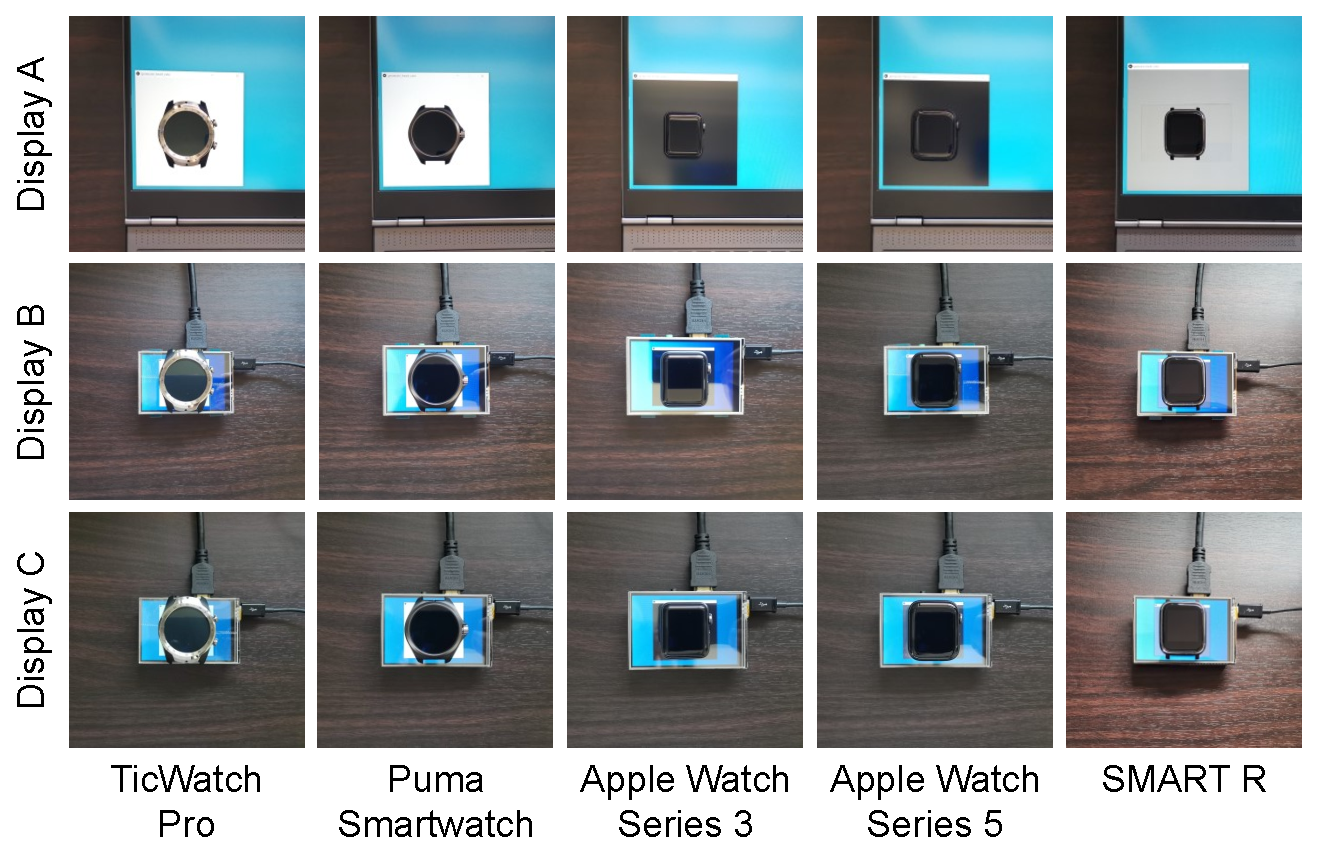
\includegraphics[width=0.75\linewidth]{figures/smartwatches.eps}
  \caption{Smartwatches and displays in the experiment.}
  \label{fig:smartwatches}
\end{figure}

\begin{figure}[!t]
  \centering
  \includegraphics[width=0.75\linewidth]{figures/flexible.eps}
  \caption{Appearance of the flexible display.}
  \label{fig:flexible}
\end{figure}


\begin{table*}[!t]
  \centering
  \caption{Error of the heart rate obtained by TicWatch Pro, PUMA Smartwatch, Apple Watch Series 3, Apple Watch Series 5, and SMART R.}
  \begin{tabular}{c|ccc|ccc|ccc|ccc|cccc} 
  \toprule
    &\multicolumn{3}{c|}{TicWatch Pro}&\multicolumn{3}{c|}{PUMA}&\multicolumn{3}{c|}{Series 3}&\multicolumn{3}{c|}{Series 5}&\multicolumn{4}{c}{SMART R}\\
    $H_{target}$ & A & B & C & A & B & C & A & B & C & A & B & C & A & B & C & D\\    \midrule
    60 & -1.7 & -1.4 & -1.4 & -1.7 & -1.4 & -1.4 & 0.4 & 1.0 & -0.2 & 58.2 & 0.1 & -0.1 & -1.7 & -1.7 & -1.0 & 1.0\\
    65 & -1.8 & -1.4 & -1.3 & -1.8 & -1.4 & -1.3 & 0.6 & 0.1 & -0.1 & 16.1 & -0.4 & 0.1 & -1.3 & -1.7 & -1.7 & -1.7\\
    70 & -1.8 & -2.1 & -1.2 & -1.8 & -2.1 & -1.2 & 0.1 & 2.0 & 0.0 & 1.6 & 2.4 & 0.1 & -1.0 & -1.3 & -1.0 & -1.0\\
    75 & -2.2 & -1.6 & -1.5 & -2.2 & -1.6 & -1.5 & 0.0 & 2.8 & -0.6 & 0.8 & 0.1 & -0.2 & -2.0 & -2.0 & -1.7 & -0.3\\
    80 & -2.0 & -1.5 & -1.1 & -2.0 & -1.5 & -1.1 & -0.5 & 1.0 & -0.5 & 1.2 & 0.9 & -0.4 & -1.0 & -2.0 & -2.0 & 0.0\\
    85 & -1.8 & -1.5 & -1.6 & -1.8 & -1.5 & -1.6 & -5.4 & -0.7 & -0.6 & -0.6 & -1.0 & -0.9 & -1.7 & -1.7 & -2.0 & -0.3\\
    90 & -2.0 & -1.7 & -1.0 & -2.0 & -1.7 & -1.0 & -0.6 & -1.3 & -0.6 & 4.3 & -1.0 & -0.9 & -2.3 & -2.0 & -2.3 & -1.0\\
    95 & -2.0 & -1.2 & -1.1 & -2.0 & -1.2 & -1.1 & -1.5 & -0.5 & -1.0 & -0.1 & -0.3 & -1.1 & -1.7 & -1.3 & -2.3 & 0.0\\
    100 & -1.9 & -1.5 & -1.4 & -1.9 & -1.5 & -1.4 & -0.7 & -1.1 & -0.7 & -0.2 & -7.3 & -0.8 & -3.0 & -3.0 & -2.7 & 0.0\\
    \midrule
    Average & -1.9 & -1.5 & -1.3 & -1.9 & -1.5 & -1.3 & -0.8 & 0.4 & -0.5 & 9.0 & -0.7 & -0.5 & -1.7 & -1.9 & -1.9 & -1.1\\
    \bottomrule
  \end{tabular}
  \label{tab:result}
\end{table*}



%Although Display B was equipped with a function to adjust the brightness, all experiments were conducted with the brightness set to maximum. 
HDMI was used to connect Display B or C to the laptop running the display control program. The flexible display blinks by switching the potential direction applied to the terminals. We implemented a system to realize the proposed method described in Section \ref{sec:method} using a microcomputer, Arduino Uno R3. This microcontroller can control the output voltage by pulse width modulation (PWM). %We connected the PWM output terminals of the Arduino to Terminals 1 and 2 of the Flexible Display. 
The Arduino receives the target heart rate from Python running on a computer connected to it, and changes the voltage to the display. The color of the display becomes darker when higher voltage is applied to the electrode 1, and lighter when higher voltage is applied to the electrode 2. The voltage of each electrode was switched between LOW and HIGH every $30/H_{target}$ seconds to let the smartwatch measures the target heart rate.
% \begin{equation*}
%   \begin{split}
%   Colors = \left(
%   \begin{tabular}{l}
%   $Terminal_{1} = [5, 0] (V)$ \\
%   $Terminal_{2} = [0, 5] (V)$
%   \end{tabular}
%   \right)
%   \end{split}
% \end{equation*}
% This is a sequence of numerical values of the voltage change given to the terminals. The system simultaneously switches the voltage applied to Terminal 1 and 2 according to the above sequence. The interval between switching voltages follows $T$[s], which is calculated from equation (\ref{eqn:wait}). Here, $len(Colors)$ is 2.\par

To obtain the correct heart rate, a 2-mm acrylic plate was placed between the display and a smartwatch in some combinations of the display and smartwatch. The smartwatches were placed on the display and the target heart rate was set to the display drawing program. The target heart rate was tested from 60 to 100 beats per minute (bpm) in increments of 5, which is the rage of the average heart rate for adults\cite{average_heart_rate}. For wearOS and watchOS smartwatches, heart rate was recorded for 60 seconds and averaged measurement was used for the evaluation. For the originalOS smartwatch, heart rate was recorded once after 30 seconds due to logging software limitation. Heart rate measurement were conducted three times for each condition.



% % 4.3.1
% \subsubsection{Wear OS Smartwatch}
% The display drawing program implemented in Section \ref{subsec:software} and the smartwatch application implemented in Section \ref{subsec:wearos} are used to collect the data. The data acquisition was done in the following flow. First, we launch the smartwatch application we implemented. Next, we run the display drawing program and start drawing the display at an appropriate heart rate. In this state, we place the smartwatch on the display and make sure that the heart rate is updated near the set value. After the placement is completed, we enter the target heart rate into the standard input of the display drawing program. Then, we press the ``RECORD'' button of the smartwatch application. We acquired data while increasing the target heart rate in increments of 5 from 60 to 100 beats per minute, the average heart rate for adults\cite{average_heart_rate}. This process is performed for three sets. The above process was used to acquire data using three displays.

% % 4.3.2
% \subsubsection{Apple Watch}
% To collect the data, we used the display drawing program implemented in Section \ref{subsec:software} and the heart rate acquisition application that comes standard with Apple Watch. The data acquisition was done in the following flow. First, we place the smartwatch on the display. Next, we run the display drawing program and start drawing the display with the target heart rate of 60, and launch the Apple Watch heart rate acquisition application. The acquisition of the heart rate starts automatically. When the data acquisition is finished, Apple Watch screen turns off. Then, we run the display drawing program and start drawing the display with the target heart rate of 65, and tap the screen of Apple Watch. The acquisition of the heart rate starts automatically. We acquired data while increasing the target heart rate in increments of 5 from 60 to 100 beats per minute, the average heart rate for adults\cite{average_heart_rate}. This process is performed for three sets. The above process was used to acquire data using three displays.


% % 4.3.3
% \subsubsection{Original OS Smartwatch}
% \label{subsubsec:original_collect}
% To collect the data, we used the display drawing program implemented in Section \ref{subsec:software} and ``WearHealth'' application. The data acquisition was done in the following flow. First, we place the smartwatch on the display. Next, we run the display drawing program and start drawing the display with the target heart rate of 60, and start acquiring the heart rate data using ``WearHealth'' application. After 30 seconds of data acquisition from the smartwatch, the final heart rate value acquired is displayed on the application. We acquired data while increasing the target heart rate in increments of 5 from 60 to 100 beats per minute, the average heart rate for adults\cite{average_heart_rate}. This process is performed for three sets. The above process was used to acquire data using four displays.


% 4.4
\subsection{Results and Discussion}
The error of the measured heart rate is calculated by subtracting the measurement from the target. The results of the evaluation experiment using TicWatch Pro, PUMA Smartwatch, Apple Watch Series 3, Apple Watch Series 5, and SMART R are shown in \tabref{result}. This result is the average of three sets. 
Zero means that the heart rate is same as the target heart rate, and minus means that the heart rate is smaller. Also, the average of the errors is shown for each display.



% 4.4.1
\subsubsection{WearOS Smartwatch}
%The error of the measured heart rate is calculated by subtracting the measurement from the target. The results of the evaluation experiment using TicWatch Pro and PumaSmartwatch are shown in \tabref{wearOS}. This result is the average of three sets. Zero means that the heart rate is same as the target heart rate, and minus means that the heart rate is smaller. Also, ``Average'' is the average of the errors for each display. 
%The sampling rate for heart rate data acquisition is approximately 1 Hz. 
%The conditions under which the data was acquired are shown in \tabref{ticwatch_params} and \tabref{puma_params}. 
The results showed that the heart rate could be input into the smartwatch within an error of less than -3 bpm. In both wearOS smartwatch results, the average error is smaller for Display A, B, and C in that order. This suggests that differences in performance, such as display brightness and refresh rate, may affect the generated heart rate. In the future, we need to conduct evaluation experiments using more displays to find displays with smaller errors.



% \begin{table}[!t]
%   \centering
%   \caption{Conditions when acquiring heart rate with TicWatch Pro.}
%   \begin{tabular}{c|c|c|c} \hline\hline
%     Conditions & Display A & Display B & Display C \\ \hline
%     $L$ & 20 & 20 & 20 \\
%     $SCALE$ & 30 & 30 & 30 \\
%     $BASE$ & 225 & 225 & 225 \\
%     Acrylic plate & $\times$ & $\bigcirc$ & $\bigcirc$ \\ \hline
%   \end{tabular}
%   \label{tab:ticwatch_params}
% \end{table}

% \begin{table}[!t]
%   \centering
%   \caption{Conditions when acquiring heart rate with PumaSmartwatch.}
%   \begin{tabular}{c|c|c|c} \hline\hline
%     Conditions & Display A & Display B & Display C \\ \hline
%     $L$ & 20 & 20 & 20 \\
%     $SCALE$ & 30 & 30 & 30 \\
%     $BASE$ & 225 & 225 & 225 \\
%     Acrylic plate & $\times$ & $\times$ & $\times$ \\ \hline
%   \end{tabular}
%   \label{tab:puma_params}
% \end{table}

% \begin{table}[!t]
%   \centering
%   \caption{Error of the heart rate obtained by TicWatch Pro and PumaSmartwatch.}
%   \begin{tabular}{c|ccc|ccc} 
%   \toprule
%     &\multicolumn{3}{c|}{TicWatch Pro}&\multicolumn{3}{c}{PumaSmartwatch}\\
%     $H_{target}$ & A & B & C & A & B & C\\
%     \midrule
%     60 & -1.7 & -1.4 & -1.4 & -1.7 & -1.4 & -1.4 \\
%     65 & -1.8 & -1.4 & -1.3 & -1.8 & -1.4 & -1.3 \\
%     70 & -1.8 & -2.1 & -1.2 & -1.8 & -2.1 & -1.2 \\
%     75 & -2.2 & -1.6 & -1.5 & -2.2 & -1.6 & -1.5 \\
%     80 & -2.0 & -1.5 & -1.1 & -2.0 & -1.5 & -1.1 \\
%     85 & -1.8 & -1.5 & -1.6 & -1.8 & -1.5 & -1.6 \\
%     90 & -2.0 & -1.7 & -1.0 & -2.0 & -1.7 & -1.0 \\
%     95 & -2.0 & -1.2 & -1.1 & -2.0 & -1.2 & -1.1 \\
%     100 & -1.9 & -1.5 & -1.4 & -1.9 & -1.5 & -1.4 \\
%     \midrule
%     Average & -1.9 & -1.5 & -1.3 & -1.9 & -1.5 & -1.3 \\
%     \bottomrule
%   \end{tabular}
%   \label{tab:wearOS}
% \end{table}

% \begin{table}[!t]
%   \centering
%   \caption{Error between the set target heart rate and the heart rate obtained by TicWatch Pro.}
%   \begin{tabular}{c|c|c|c} \hline\hline
%     $H_{target}$ & Display A & Display B & Display C \\ \hline
%     60 & -1.7 & -1.4 & -1.4 \\
%     65 & -1.8 & -1.4 & -1.3 \\
%     70 & -1.8 & -2.1 & -1.2 \\
%     75 & -2.2 & -1.6 & -1.5 \\
%     80 & -2.0 & -1.5 & -1.1 \\
%     85 & -1.8 & -1.5 & -1.6 \\
%     90 & -2.0 & -1.7 & -1.0 \\
%     95 & -2.0 & -1.2 & -1.1 \\
%     100 & -1.9 & -1.5 & -1.4 \\ \hline
%     Average & -1.9 & -1.5 & -1.3 \\ \hline
%   \end{tabular}
%   \label{tab:ticwatch_result}
% \end{table}

% \begin{table}[!t]
%   \centering
%   \caption{Error between the set target heart rate and the heart rate obtained by PumaSmartwatch.}
%   \begin{tabular}{c|c|c|c} \hline\hline
%     $H_{target}$ & Display A & Display B & Display C \\ \hline
%     60 & -1.1 & -1.8 & -0.8 \\
%     65 & -1.3 & -1.6 & -0.5 \\
%     70 & -1.9 & -1.9 & -0.5 \\
%     75 & -3.0 & -1.6 & -0.6 \\
%     80 & -2.4 & -1.5 & -1.6 \\
%     85 & -2.4 & -1.7 & -1.7 \\
%     90 & -2.5 & -1.7 & -1.8 \\
%     95 & -2.7 & -1.4 & -2.0 \\
%     100 & -2.7 & -2.1 & -2.0 \\ \hline
%     Average & -2.2 & -1.7 & -1.3 \\ \hline
%   \end{tabular}
%   \label{tab:puma_result}
% \end{table}


% 4.4.2
\subsubsection{WatchOS Smartwatch}
%In the experiment using Apple Watch, the heart rate data was acquired using the application provided by the manufacturer, so the data acquisition time and calibration time could not be set. However, the data is time-stamped. Observing the acquired data, it was found that the data was acquired for approximately 160 seconds at maximum, considering the time when the first sample was acquired as 0. However, it may include data acquisition in the background while the display is off. 30 seconds from the time when the first sample was obtained was used as calibration time, and the data obtained during that time was not used. The time 30 seconds after the first sample was obtained was let to 0, and only the data obtained during the next 60 seconds was used for evaluation. If there were no data acquired after the calibration time, only the last data acquired was used.\par
%The error of the heart rate obtained with the Apple Watch Series 3 and Series 5 are shown in \tabref{watchOS}. The result is the average of three sets.
%We calculated the error between the set target heart rate and the heart rate. 0 means that the heart rate is consistent with the target heart rate, and minus means that the heart rate is insufficient. Also, ``Average'' is the average of the errors for each display. The sampling rate for heart rate acquisition with Apple Watch varied with each acquisition. ``MAX'' is the maximum number of data obtained in that acquisition cycle, and ``MIN'' is the minimum number. This number of data does not include the data obtained during calibration. The conditions under which the data was acquired are shown in \tabref{series3_params} and \tabref{series5_params}. The results of the evaluation experiment using Apple Watch Series 3 are shown in \tabref{series3_result_1st}, \tabref{series3_result_2nd}, and \tabref{series3_result_3rd}. The results of the evaluation experiment using Apple Watch Series 5 are shown in \tabref{series5_result_1st}, \tabref{series5_result_2nd}, and \tabref{series5_result_3rd}. 
The results showed that Using Display C, the heart rate could be input into the Apple Watch within an error of 0.1 to -1.1 bpm. On the other hand, when using Display A and B, it was not possible to obtain the correct heart rate under some conditions. In particular, when the target heart rate was set to 60 with the combination of Apple Watch Series 5 and Display A, the correct heart rate was not obtained even once. However, there are many cases where the heart rate is obtained correctly. In the future, it is necessary to clarify the conditions under which the heart rate cannot be obtained correctly.

% \begin{table}[!t]
%   \centering
%   \caption{Conditions when acquiring heart rate with Apple Watch Series 3.}
%   \begin{tabular}{c|c|c|c} \hline\hline
%     Conditions & Display A & Display B & Display C \\ \hline
%     $L$ & 10 & 10 & 10 \\
%     $SCALE$ & 20 & 40 & 40 \\
%     $BASE$ & 0 & 0 & 0 \\
%     Acrylic plate & $\times$ & $\times$ & $\times$ \\ \hline
%   \end{tabular}
%   \label{tab:series3_params}
% \end{table}

% \begin{table}[!t]
%   \centering
%   \caption{Conditions when acquiring heart rate with Apple Watch Series 5.}
%   \begin{tabular}{c|c|c|c} \hline\hline
%     Conditions & Display A & Display B & Display C \\ \hline
%     $L$ & 10 & 10 & 10 \\
%     $SCALE$ & 20 & 50 & 40 \\
%     $BASE$ & 0 & 50 & 20 \\
%     Acrylic plate & $\times$ & $\bigcirc$ & $\times$ \\ \hline
%   \end{tabular}
%   \label{tab:series5_params}
% \end{table}

% \begin{table}[!t]
%   \centering
%   \caption{Error of the heart rate obtained by Apple Watch Series 3 and Series 5.}
%   \begin{tabular}{c|ccc|ccc} 
%   \toprule
%     &\multicolumn{3}{c|}{Series 3}&\multicolumn{3}{c}{Series 5}\\
%     $H_{target}$ & A & B & C & A & B & C\\
%     \midrule
%     60 & 0.4 & 1.0 & -0.2 & -1.7 & -1.4 & -1.4 \\
%     65 & 0.6 & 0.1 & -0.1 & -1.8 & -1.4 & -1.3 \\
%     70 & 0.1 & 2.0 & 0.0 & -1.8 & -2.1 & -1.2 \\
%     75 & 0.0 & 2.8 & -0.6 & -2.2 & -1.6 & -1.5 \\
%     80 & -0.5 & 1.0 & -0.5 & -2.0 & -1.5 & -1.1 \\
%     85 & -5.4 & -0.7 & -0.6 & -1.8 & -1.5 & -1.6 \\
%     90 & -0.6 & -1.3 & -0.6 & -2.0 & -1.7 & -1.0 \\
%     95 & -1.5 & -0.5 & -1.0 & -2.0 & -1.2 & -1.1 \\
%     100 & -0.7 & -1.1 & -0.7 & -1.9 & -1.5 & -1.4 \\
%     \midrule
%     Average & -0.8 & 0.4 & -0.5 & -1.9 & -1.5 & -1.3 \\
%     \bottomrule
%   \end{tabular}
%   \label{tab:watchOS}
% \end{table}

% \begin{table}[!t]
%   \centering
%   \caption{[1st] Error between the set target heart rate and the heart rate obtained by Apple Watch Series 3.}
%   \begin{tabular}{c|c|c|c} \hline\hline
%     $H_{target}$ & Display A & Display B & Display C \\ \hline
%     60 & 0.0 & 0.8 & -0.3 \\
%     65 & 1.2 & 0.7 & -0.3 \\
%     70 & 0.0 & 1.0 & -0.2 \\
%     75 & 0.0 & 1.4 & -0.8 \\
%     80 & -0.7 & 0.7 & -0.6 \\
%     85 & -0.4 & -0.6 & -0.9 \\
%     90 & 0.0 & -1.5 & -1.0 \\
%     95 & -1.4 & -0.3 & -1.0 \\
%     100 & -1.0 & -1.2 & -0.8 \\ \hline
%     Average & -0.2 & 0.1 & -0.7 \\ \hline \hline
%     MIN & 2 & 6 & 11 \\ \hline
%     MAX & 9 & 13 & 12 \\ \hline
%   \end{tabular}
%   \label{tab:series3_result_1st}
% \end{table}

% \begin{table}[!t]
%   \centering
%   \caption{[2nd] Error between the set target heart rate and the heart rate obtained by Apple Watch Series 3.}
%   \begin{tabular}{c|c|c|c} \hline\hline
%     $H_{target}$ & Display A & Display B & Display C \\ \hline
%     60 & 0.8 & 1.1 & -0.3 \\
%     65 & 0.0 & -0.4 & -0.2 \\
%     70 & 0.0 & 2.2 & -0.1 \\
%     75 & 0.0 & 3.6 & -0.6 \\
%     80 & -0.5 & 1.2 & -0.3 \\
%     85 & -0.7 & -0.9 & -0.3 \\
%     90 & -1.0 & -1.2 & -0.3 \\
%     95 & -1.2 & -0.8 & -1.0 \\
%     100 & -1.2 & -1.3 & -0.5 \\ \hline
%     Average & -0.4 & 0.4 & -0.4 \\ \hline \hline
%     MIN & 2 & 9 & 11 \\ \hline
%     MAX & 10 & 13 & 13 \\ \hline
%   \end{tabular}
%   \label{tab:series3_result_2nd}
% \end{table}

% \begin{table}[!t]
%   \centering
%   \caption{[3rd] Error between the set target heart rate and the heart rate obtained by Apple Watch Series 3.}
%   \begin{tabular}{c|c|c|c} \hline\hline
%     $H_{target}$ & Display A & Display B & Display C \\ \hline
%     60 & 0.5 & 1.2 & -0.2 \\
%     65 & 0.7 & 0.0 & 0.2 \\
%     70 & 0.3 & 2.6 & 0.2 \\
%     75 & 0.0 & 3.4 & -0.3 \\
%     80 & -0.3 & 1.2 & -0.5 \\
%     85 & -15.0 & -0.5 & -0.6 \\
%     90 & -0.8 & -1.1 & -0.5 \\
%     95 & -2.0 & -0.2 & -0.9 \\
%     100 & 0.0 & -0.8 & -0.7 \\ \hline
%     Average & -1.9 & 0.6 & -0.4 \\ \hline \hline
%     MIN & 1 & 8 & 12 \\ \hline
%     MAX & 13 & 13 & 13 \\ \hline
%   \end{tabular}
%   \label{tab:series3_result_3rd}
% \end{table}

% \begin{table}[!t]
%   \centering
%   \caption{[1st] Error between the set target heart rate and the heart rate obtained by Apple Watch Series 5.}
%   \begin{tabular}{c|c|c|c} \hline\hline
%     $H_{target}$ & Display A & Display B & Display C \\ \hline
%     60 & 58.1 & 0.0 & 0.1 \\
%     65 & 4.3 & 0.0 & 0.1 \\
%     70 & 3.4 & 5.0 & 0.0 \\
%     75 & 0.0 & 0.0 & -0.3 \\
%     80 & 1.1 & 1.0 & -0.3 \\
%     85 & -0.9 & -1.0 & -0.9 \\
%     90 & 2.6 & -1.7 & -0.8 \\
%     95 & 0.7 & -0.5 & -1.2 \\
%     100 & -0.5 & -21.0 & -1.3 \\ \hline
%     Average & 7.6 & -2.0 & -0.5 \\ \hline \hline
%     MIN & 6 & 1 & 12 \\ \hline
%     MAX & 13 & 5 & 13 \\ \hline
%   \end{tabular}
%   \label{tab:series5_result_1st}
% \end{table}

% \begin{table}[!t]
%   \centering
%   \caption{[2nd] Error between the set target heart rate and the heart rate obtained by Apple Watch Series 5.}
%   \begin{tabular}{c|c|c|c} \hline\hline
%     $H_{target}$ & Display A & Display B & Display C \\ \hline
%     60 & 58.7 & 0.4 & -0.2 \\
%     65 & 43.4 & -0.3 & 0.0 \\
%     70 & 0.5 & 1.0 & 0.2 \\
%     75 & 2.2 & 0.2 & -0.3 \\
%     80 & 2.2 & 0.7 & -0.2 \\
%     85 & -0.5 & -1.0 & -0.9 \\
%     90 & 11.0 & -1.3 & -1.0 \\
%     95 & -0.4 & -0.5 & -1.1 \\
%     100 & 1.1 & -1.0 & -0.2 \\ \hline
%     Average & 13.1 & -0.2 & -0.4 \\ \hline \hline
%     MIN & 5 & 2 & 12 \\ \hline
%     MAX & 13 & 7 & 13 \\ \hline
%   \end{tabular}
%   \label{tab:series5_result_2nd}
% \end{table}

% \begin{table}[!t]
%   \centering
%   \caption{[3rd] Error between the set target heart rate and the heart rate obtained by Apple Watch Series 5.}
%   \begin{tabular}{c|c|c|c} \hline\hline
%     $H_{target}$ & Display A & Display B & Display C \\ \hline
%     60 & 57.8 & 0.0 & -0.2 \\
%     65 & 0.6 & -1.0 & 0.1 \\
%     70 & 0.8 & 1.2 & 0.1 \\
%     75 & 0.1 & 0.0 & -0.1 \\
%     80 & 0.3 & 1.0 & -0.7 \\
%     85 & -0.4 & -1.0 & -0.8 \\
%     90 & -0.8 & 0.0 & -1.0 \\
%     95 & -0.5 & 0.0 & -1.1 \\
%     100 & -1.3 & 0.0 & -0.9 \\ \hline
%     Average & 6.3 & 0.0 & -0.5 \\ \hline \hline
%     MIN & 5 & 1 & 12 \\ \hline
%     MAX & 13 & 5 & 13 \\ \hline
%   \end{tabular}
%   \label{tab:series5_result_3rd}
% \end{table}


% 4.4.3
\subsubsection{Original OS Smartwatch}
%The error of the heart rate obtained with the SMART R are shown in \tabref{original_result}. The result is the average of three sets.
%We calculated the error between the set target heart rate and the heart rate. This result is the average of three sets. 0 means that the heart rate is consistent with the target heart rate, and minus means that the heart rate is insufficient. Also, ``Average'' is the average of the errors for each display. The conditions under which the data was acquired are shown in \tabref{original_params}. The results of the evaluation experiment using SMART R are shown in \tabref{original_result}. 
The results showed that the heart rate could be input into the smartwatch within an error of less than -3 bpm. Especially for the flexible display, the heart rate could be input into the smartwatch within an error of less than -2 bpm.


% \begin{table}[!t]
%   \centering
%   \caption{Conditions when acquiring heart rate with SMART R.}
%   \begin{tabular}{c|c|c|c} \hline\hline
%     Conditions & Display A & Display B & Display C \\ \hline
%     $L$ & 20 & 20 & 20 \\
%     $SCALE$ & 100 & 100 & 100 \\
%     $BASE$ & 0 & 0 & 0 \\
%     Acrylic plate & $\bigcirc$ & $\times$ & $\times$ \\ \hline
%   \end{tabular}
%   \label{tab:original_params}
% \end{table}

% \begin{table}[!t]
%   \centering
%   \caption{Error between the set target heart rate and the heart rate obtained by SMART R.}
%   \begin{tabular}{c|c|c|c} \hline\hline
%     $H_{target}$ & Display A & Display B & Display C \\ \hline
%     60 & -1.7 & -1.7 & -1.0 \\
%     65 & -1.3 & -1.7 & -1.7 \\
%     70 & -1.0 & -1.3 & -1.0 \\
%     75 & -2.0 & -2.0 & -1.7 \\
%     80 & -1.0 & -2.0 & -2.0 \\
%     85 & -1.7 & -1.7 & -2.0 \\
%     90 & -2.3 & -2.0 & -2.3 \\
%     95 & -1.7 & -1.3 & -2.3 \\
%     100 & -3.0 & -3.0 & -2.7 \\ \hline
%     Average & -1.7 & -1.9 & -1.9 \\ \hline
%   \end{tabular}
%   \label{tab:original_result}
% \end{table}


% 4.5
%\subsection{Flexible Display}
% The evaluation was conducted using a lightweight and flexible display designed to be worn on the body.
% % フレキシブルディスプレイはこんなもんであるという説明
% The size of the lighted part of the flexible display is approximately 1cm square. The appearance of the flexible display is shown in the left side of \figref{flexible}.\par

% \begin{figure}[!t]
%   \centering
%   \includegraphics[width=1\linewidth]{figures/flexible.eps}
%   \caption{Appearance of the flexible display.}
%   \label{fig:flexible}
% \end{figure}

% The flexible display blinks by switching the potential direction applied to the terminals. We implemented a system to realize the proposed method described in Section \ref{sec:method} using a microcomputer, Arduino Uno R3. This microcontroller can control the output voltage by PWM (Pulse Width Modulation). We connected the PWM output terminals of the Arduino to Terminals 1 and 2 of the Flexible Display. The Arduino receives the target heart rate from Python running on a computer connected to it, and changes the voltage value according to the value. The color of the display becomes darker when voltage is applied to Terminal 1, and lighter when voltage is applied to Terminal 2. $Colors$ described in Section \ref{subsec:display_control} are set as follows.
% \begin{equation*}
%   \begin{split}
%   Colors = \left(
%   \begin{tabular}{l}
%   $Terminal_{1} = [5, 0] (V)$ \\
%   $Terminal_{2} = [0, 5] (V)$
%   \end{tabular}
%   \right)
%   \end{split}
% \end{equation*}
% This is a sequence of numerical values of the voltage change given to the terminals. The system simultaneously switches the voltage applied to Terminal 1 and 2 according to the above sequence. The interval between switching voltages follows $T$[s], which is calculated from equation (\ref{eqn:wait}). Here, $len(Colors)$ is 2.\par

%Since the SMART R was the only smartwatch in which the size of the PPG sensor did not exceed the size of the light-emitting part, we conducted the evaluation using only this smartwatch. Data acquisition was performed in the same flow as in Section \ref{subsubsec:original_collect}. In cases where obviously incorrect values were obtained, the data was obtained again.\par

%We calculated the error between the set target heart rate and the heart rate. This result is the average of three sets. 0 means that the heart rate is consistent with the target heart rate, and minus means that the heart rate is insufficient. Also, ``Average'' is the average of the errors for each display. The results of the evaluation experiment using SMART R are shown in \tabref{flexible_result}. 
%The results showed that when the target heart rate was between 60 and 100 beats per minute which is the average heart rate of adults, the heart rate could be input into the smartwatch within an error of less than -2 beats per minute.

% \begin{table}[!t]
%   \centering
%   \caption{Error between the set target heart rate and the heart rate obtained by SMART R.}
%   \begin{tabular}{c|c} \hline\hline
%     $H_{target}$ & Flexible Display \\ \hline
%     60 & 1.0 \\
%     65 & -1.7 \\
%     70 & -1.0 \\
%     75 & -0.3 \\
%     80 & 0.0 \\
%     85 & -0.3 \\
%     90 & -1.0 \\
%     95 & 0.0 \\
%     100 & 0.0 \\ \hline
%     Average & -1.1 \\ \hline
%   \end{tabular}
%   \label{tab:flexible_result}
% \end{table}



% % 5
% \section{Future work}
% \label{sec:future_work}

% \begin{figure}[!t]
%   \centering
%   \includegraphics[width=1\linewidth]{figures/future_work.eps}
%   \caption{A mechanism for inputting and reproducing PPG data obtained from a live body part.}
%   \label{fig:future_work}
% \end{figure}

% In the future, we will implement a mechanism that allows the wearable device to measure PPG data similar to that obtained from a live body part by using a display. In order to do so, the system needs to automatically determine the color tone of the display, so we design an appropriate generative model. We will also study miniaturization of the device, assuming that it can be attached to a body part.



% 5
\section{Conclusion}
\label{sec:conclusion}
In this paper, we proposed a method to let the PPG sensor measure an arbitrary heart rate using a display. We implemented a display drawing program and conducted an evaluation experiment using five kinds of smartwatches and four kinds of displays to confirm the effectiveness of the proposed method. As a result, the overall error between the target heart rate entered and the heart rate acquired by the smartwatch was within -3 beats per minute in most cases.\par
%In the evaluation experiment, we were able to make the smartwatch measure the target heart rate with an error of less than -3 beats per minute using the display. However, there are restrictions on the display, and there is a possibility that the acquired values may vary severely depending on the position of the wearer.\par

In the future, we will improve the reproducibility of PPG data for use in a real environment, and implement a mechanism that allows the wearable device worn on the display to measure the same PPG data by inputting PPG data obtained from a live body part. To achieve this, the system needs to continue to automatically determine the colors to be drawn on the display. Therefore, we will build a generative model that can output the color to be drawn on the display by inputting PPG data.
%In addition, we will miniaturize the device to be worn on the body part, and conduct experiments using more wearable devices.





% \section{Acknowledgments}

% Identification of funding sources and other support, and thanks to
% individuals and groups that assisted in the research and the
% preparation of the work should be included in an acknowledgment
% section, which is placed just before the reference section in your
% document.

% This section has a special environment:
% \begin{verbatim}
%   \begin{acks}
%   ...
%   \end{acks}
% \end{verbatim}
% so that the information contained therein can be more easily collected
% during the article metadata extraction phase, and to ensure
% consistency in the spelling of the section heading.

% Authors should not prepare this section as a numbered or unnumbered {\verb|\section|}; please use the ``{\verb|acks|}'' environment.

% \section{Appendices}

% If your work needs an appendix, add it before the
% ``\verb|\end{document}|'' command at the conclusion of your source
% document.

% Start the appendix with the ``\verb|appendix|'' command:
% \begin{verbatim}
%   \appendix
% \end{verbatim}
% and note that in the appendix, sections are lettered, not
% numbered. This document has two appendices, demonstrating the section
% and subsection identification method.

% \section{SIGCHI Extended Abstracts}

% The ``\verb|sigchi-a|'' template style (available only in \LaTeX\ and
% not in Word) produces a landscape-orientation formatted article, with
% a wide left margin. Three environments are available for use with the
% ``\verb|sigchi-a|'' template style, and produce formatted output in
% the margin:
% \begin{itemize}
% \item {\verb|sidebar|}:  Place formatted text in the margin.
% \item {\verb|marginfigure|}: Place a figure in the margin.
% \item {\verb|margintable|}: Place a table in the margin.
% \end{itemize}

%%
%% The acknowledgments section is defined using the "acks" environment
%% (and NOT an unnumbered section). This ensures the proper
%% identification of the section in the article metadata, and the
%% consistent spelling of the heading.
% \begin{acks}
% To Robert, for the bagels and explaining CMYK and color spaces.
% \end{acks}

%%
%% The next two lines define the bibliography style to be used, and
%% the bibliography file.
\bibliographystyle{ACM-Reference-Format}
\bibliography{references}

%%
%% If your work has an appendix, this is the place to put it.
% \appendix

% \section{Research Methods}

% \subsection{Part One}

% Lorem ipsum dolor sit amet, consectetur adipiscing elit. Morbi
% malesuada, quam in pulvinar varius, metus nunc fermentum urna, id
% sollicitudin purus odio sit amet enim. Aliquam ullamcorper eu ipsum
% vel mollis. Curabitur quis dictum nisl. Phasellus vel semper risus, et
% lacinia dolor. Integer ultricies commodo sem nec semper.

% \subsection{Part Two}

% Etiam commodo feugiat nisl pulvinar pellentesque. Etiam auctor sodales
% ligula, non varius nibh pulvinar semper. Suspendisse nec lectus non
% ipsum convallis congue hendrerit vitae sapien. Donec at laoreet
% eros. Vivamus non purus placerat, scelerisque diam eu, cursus
% ante. Etiam aliquam tortor auctor efficitur mattis.

% \section{Online Resources}

% Nam id fermentum dui. Suspendisse sagittis tortor a nulla mollis, in
% pulvinar ex pretium. Sed interdum orci quis metus euismod, et sagittis
% enim maximus. Vestibulum gravida massa ut felis suscipit
% congue. Quisque mattis elit a risus ultrices commodo venenatis eget
% dui. Etiam sagittis eleifend elementum.

% Nam interdum magna at lectus dignissim, ac dignissim lorem
% rhoncus. Maecenas eu arcu ac neque placerat aliquam. Nunc pulvinar
% massa et mattis lacinia.

\end{document}
\endinput
%%
%% End of file `sample-authordraft.tex'.
